\renewcommand{\chaptername}{Introduction}
\chapter*{Introduction}
\setcounter{page}{1}
\pagenumbering{arabic}
\addcontentsline{toc}{chapter}{Introduction}


\shorthandoff{-} 

\section{Taxonomy and characteristics of \tax{Escherichia coli}}
\hspace*{0,5cm} Domain: \hspace{0,5cm} \tax{Bacteria}\\%
\hspace*{1,5cm} Phylum: \hspace{0,5cm} \tax{Proteobacteria}\\%
\hspace*{2,5cm} Class: \hspace{0,5cm} \tax{Gammaproteobacteria}\\%
\hspace*{3,5cm} Order: \hspace{0,5cm} \tax{Enterobacteriales}\\%
\hspace*{4,5cm} Family: \hspace{0,5cm} \tax{Enterobacteriaceae}\\%

% 2018.07.12
% not sure this should be the top section. the fact that it's e. coli si not critical
% just start at section 0.2? 
\tax{E. coli} is Gram-negative bacterium with facultative anaerobic metabolism.
Since its first isolation from infant faeces by Theodor Escherich in 1885 \cite{friedmann2006escherich}, this organism was found in gastrointestinal tract of other warm-blooded animals and reptiles \cite{gopee2000longitudinal} as well as in environmental samples such as soil or water.
\tax{E. coli} is known to be a part of normal intestine microbiota.
On the other hand extraintestinal infections caused by this bacterium are common and some strains (e.g. STEC) even possess virulence factors leading to heavy intestinal infections when expressed \cite{allocati2013escherichia}.

\section{Transcription and memory}
%%%A bacterial genome consists of hundreds and thousands of genes, but not all of them are active at all the time.
%%%Gene expression changes during a cell cycle, when a nutrient source is altered or if surrounding conditions begin to be unfavourable.
It is vital for a living cell to sense what is happening in the environment it is present at and react accordingly by transcription initiation or silencing of appropriate genes.
Some studies has shown that cells with the same genetic background might react differently or at a different rate to the same stimulus based on their and their ancestors recent experience \cite{mathis2017asymmetric, ronin2017long}.
Such ability is advantageous especially if the change in the conditions is predictable and repeats periodically.

% 2018.07.12
% might need a nice transition from 0.2 to 0.2.1 0.2 could be expanded a bit?
% I (or someone else) can help with grammar corrections later
\subsection{Cellular responses}
Ability to sense changes in both surrounding and intracellular environment and to respond to them is essential for every living cell.
Important decision makings rely on the information acquired this way, for example if the cell should start dividing, whether to stay in actual place or to move elsewhere or if as a pathogen start to produce virulence factors or not \cite{gottesman2003proteolysis, sourjik2012responding, cui2018novel}.
To manage and orchestrate all possible responses to multiple signals cells evolved a network of extra- and intracellular signaling pathways.
As I focus on transcriptional responses the following text covers mostly these cases.
However, regulation on translation level or control of activity of existing proteins occur in bacteria as well.

\subsubsection{Direct signaling pathways}
When a signal molecule is imported through cell membrane into cytosol or is produced by the cell and subsequently interacts with gene regulatory protein we can talk about direct signaling.
This is often the case in the regulation of carbohydrate catabolism and amino acid biosynthesis genes \cite{charlier1992arginine, weickert1992isorepressor, pittard1996various, wheatley2013structural}.
Two simple models are described below.

% 2018.07.12
% "producing heaps" is a bit colloquial. stay slightly more formal in your writing
Cells avoid wasteful production of proteins which are not used at all the time.
For instance, there is no sense in producing heaps of enzyme hydrolysing lactose (lacZ) if no lactose is present.
To achieve this \tax{E. coli} expresses \tax{lac} repressor (LacI) \cite{hudson1990co}.
However, \tax{lac} operon transcription is required if lactose is present in the media.
% 2018.07.12 not *required* per se, but *desired*
Here \tax{lac} operon inducers take a turn.
% 2018.07.12 don't really like IPTG as a *true* inducer as it's not a substance E. coli would encounter in nature
Lactose analogue IPTG and allolactose are true inducers of \tax{lac} operon as lactose permease imports them into the cell where they bind directly to the repressor LacI.
Lactose itself has to modified to its isomer allolactose by $\beta$-galactosidase (LacZ) at first \cite{jobe1972lac, wheatley2013structural}.
LacI binding to promoter DNA is then released triggering \tax{lacZYA} expression (Fig. \ref{dir}\textcolor{red}{a}) if an simultaneous activation by general regulatory protein CRP occurs \cite{hudson1990co, clark2005molecular}.

\begin{figure}[ht]
  \centering
  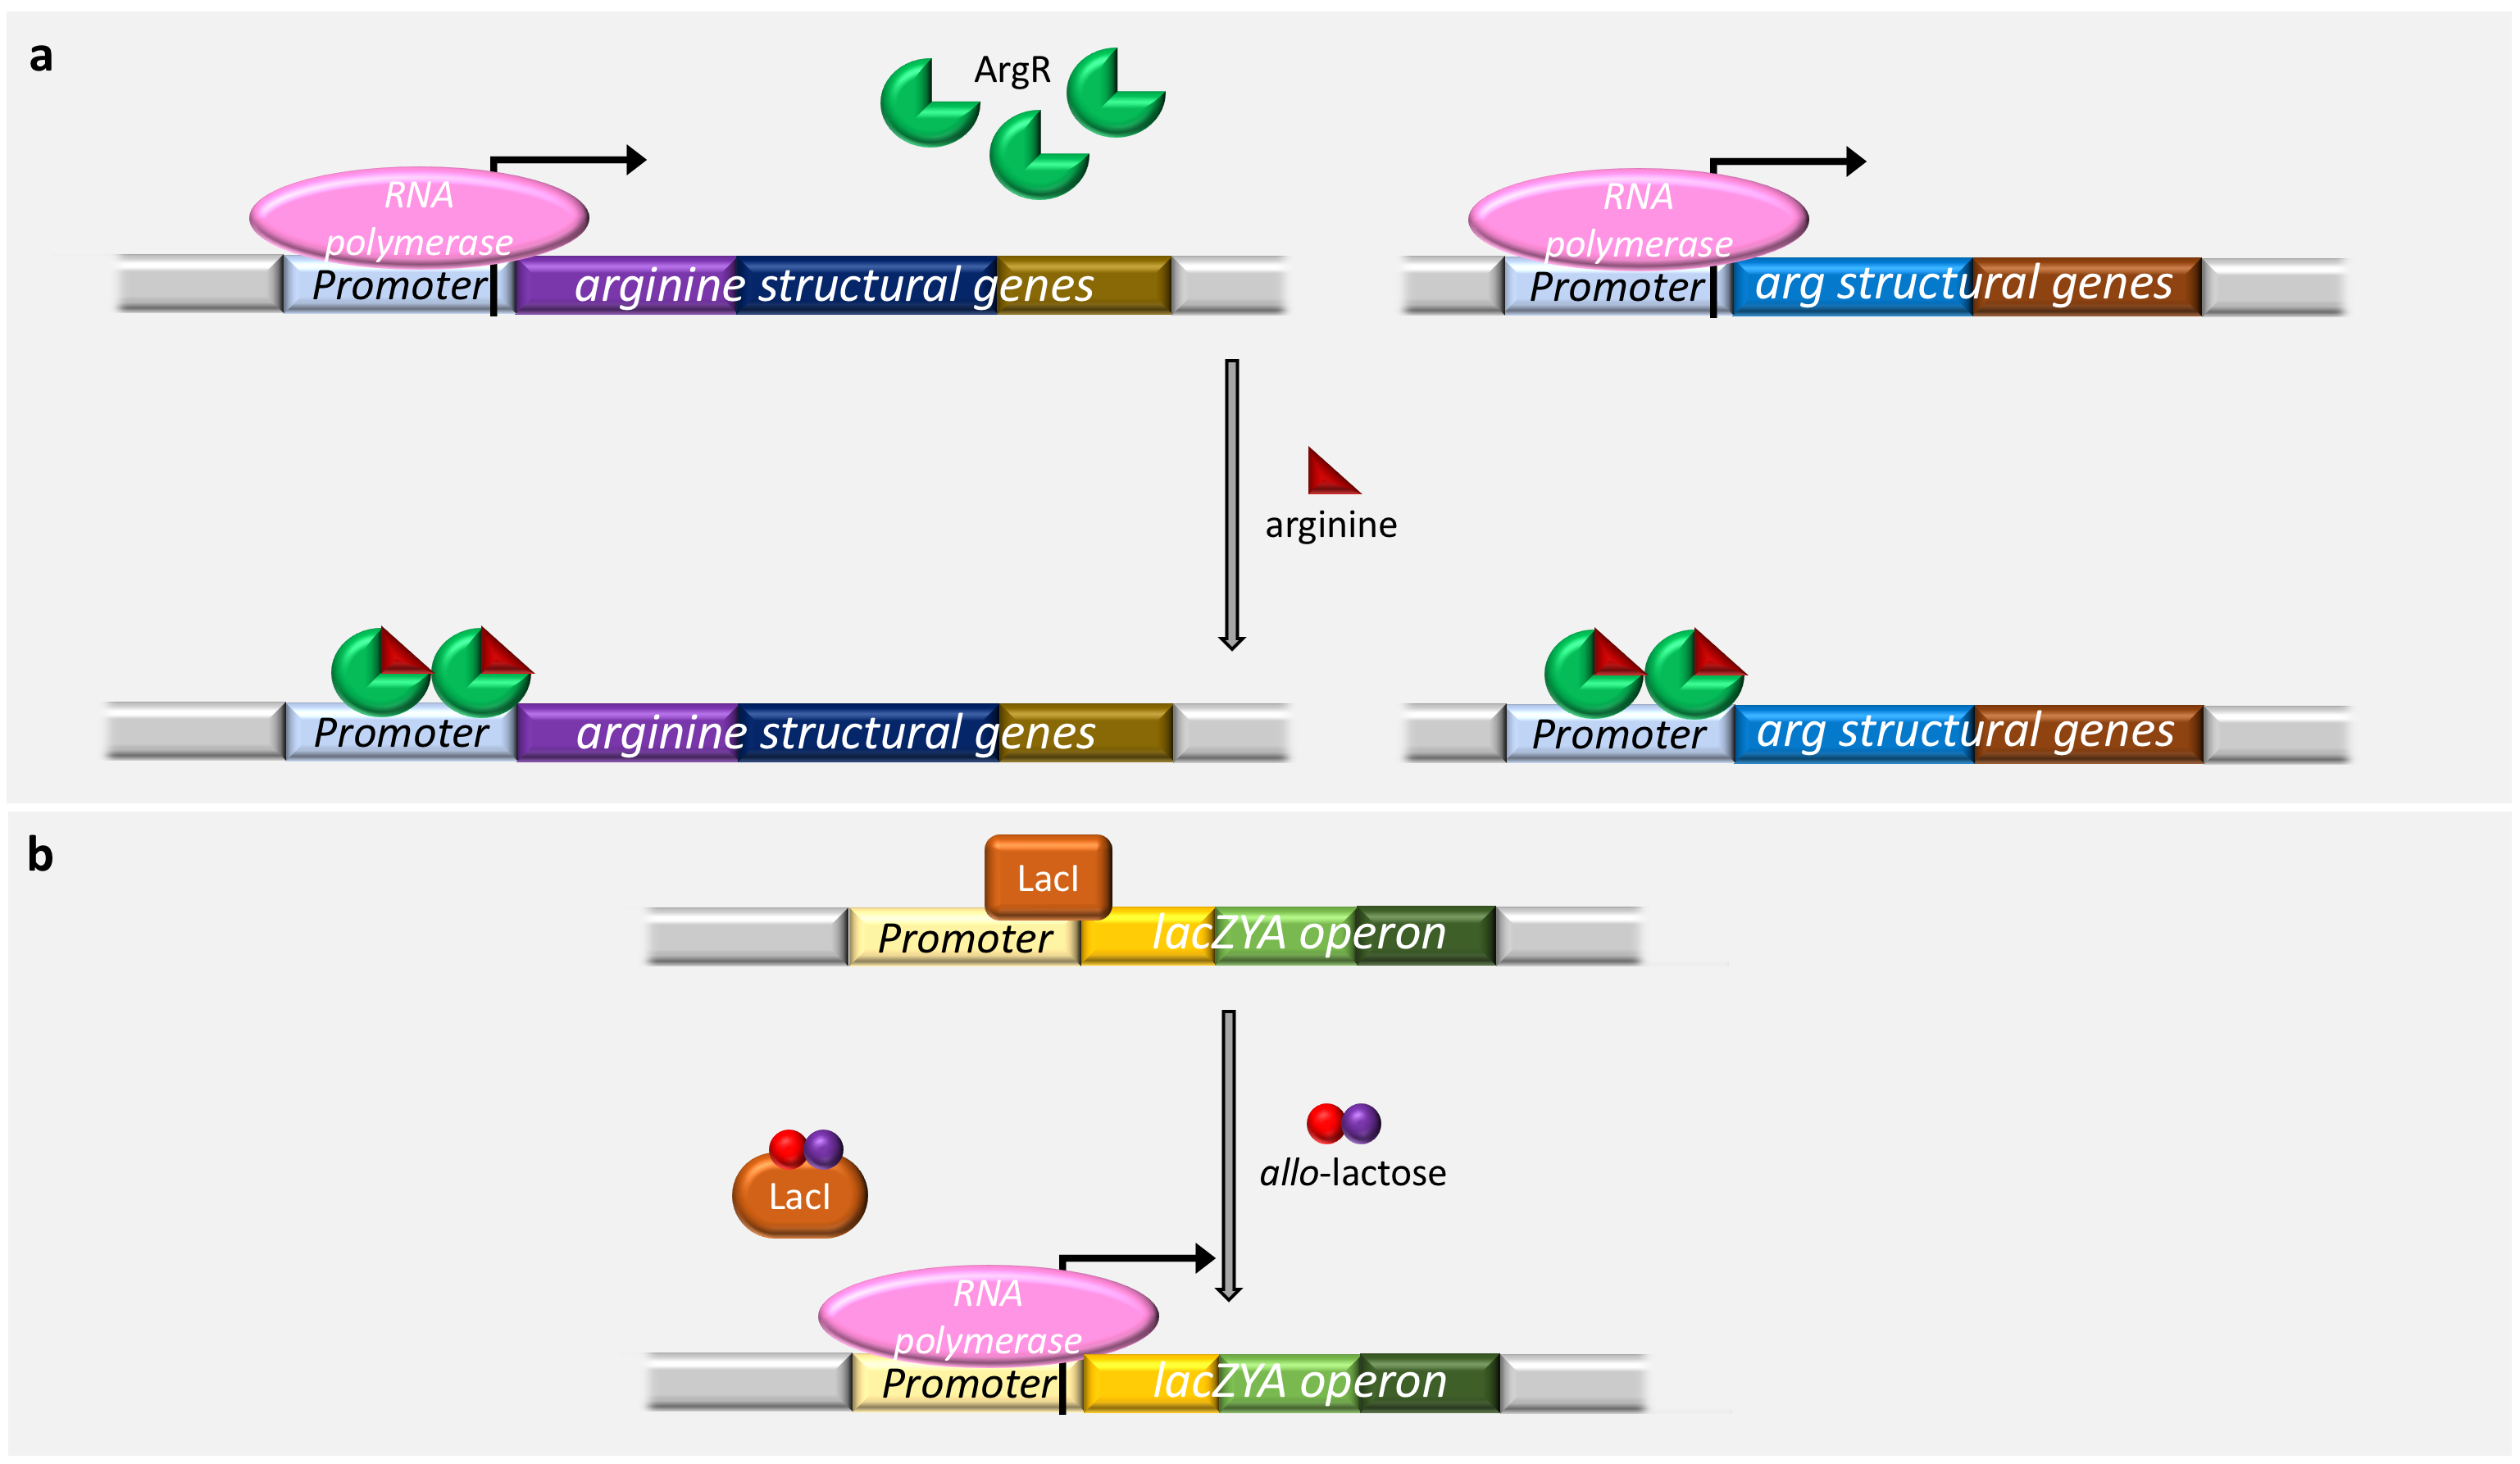
\includegraphics[scale=0.27]{text/Pictures/DirectSignaling.png}
	\caption{Scheme of direct signaling. \textbf{a} if \tax{lac} operon inducer (allolactose) is present it binds to LacI repressor and induces \tax{lac} operon transcription. \textbf{b} expression of arginine structural genes is co-repressed by arginine itself, because without it ArgR repressor cannot bind to DNA.}
	\label{dir}
\end{figure}

% 2018.07.12 you need a transition here to talking about arginine, e.g. "For other metabolic pathways..."
% you might also talk about other direct inducers that are not metabolic, e.g. SOS/lexA/recA
Contrary to galactoside induction of \tax{lac} operon, arginine acts as a co-repressor of its own biosynthesis (Fig. \ref{dir}\textcolor{red}{b}).
This means that when a bacterium does not have enough of this amino acid available for protein production the transcription of arginine genes is active \cite{charlier2004biosynthesis, caldara2006arginine}.
On the other hand, when arginine is abundant in the culture medium and thus in the cell, there is no need to make more of it.
The cell has ArgR repressor present in cytosol but ArgR itself cannot bind to DNA and inhibit transcription in the arginine absence \cite{clark2005molecular, caldara2006arginine}.
However when there is plenty of arginine in the cell it binds to ArgR and as a co-repressor inhibits expression of arginine structural genes binding to an appropriate promoter \cite{charlier1992arginine, charlier2004biosynthesis, clark2005molecular}.

\subsubsection{Two-component system}
% 2018.07.12 this intro paragraph is quite confusing. Start instead with something similar to the next paragraph?
Direct signaling is straight forward, but an external signal molecule is not always imported into the cell.
Instead covalent modifications of sensory protein by a chemical group are used in some cases \cite{ninfa1986covalent, falke1997two}.
This is mostly the case of regulation of genes involved in stress response.
But it it not limited only to stress responses as the two-component system represents a dominant and versatile form of bacterial sense-response processes \cite{karniol2004hwe, kaczmarczyk2014complex, cui2018novel}.
It utilizes phosphate as a chemical group, however other groups can be used for cell signalling as well e.g. methyl, acetyl, AMP or even redox reactions \cite{kim2002oxyr, chaparro2010toxt, wang2010acetylation, you2013coordination}.

A classic two-component system consists of a transmembrane sensory kinase which is autophosphorylated at its histidine residue after receiving physical or chemical signal from the environment (Fig. \ref{two}\textcolor{red}{a}).
To be able to phosphorylate itself the kinase requires ATP or other phosphate donor.
Next, the phosphorylated kinase transfers the phosphate group to its partner regulatory protein enabling its activity, most often DNA-binding \cite{lynch2012prioritization, gao2015temporal, cui2018novel}.
This protein receives the phosphate to its aspartate residue and might act as both gene repressor and/or activator.
Alternatively, the output of the two-component system can be a modification of biochemical activity of target proteins or RNAs instead or on the top of the change in gene expression \cite{shu2002antar, chambonnier2016hybrid}.

The described kinases and cognate regulatory proteins do not necessarily need to be separated units.
Proteins with histidine kinase domains connected to aspartate domains of DNA-binding proteins are known.
These hybrid systems are usually located in cell membrane with their sensory domains in periplasmic space (Fig. \ref{two}\textcolor{red}{b}) \cite{lynch2012prioritization, hirano2013regulon}.

\begin{figure}[h!]
  \centering
  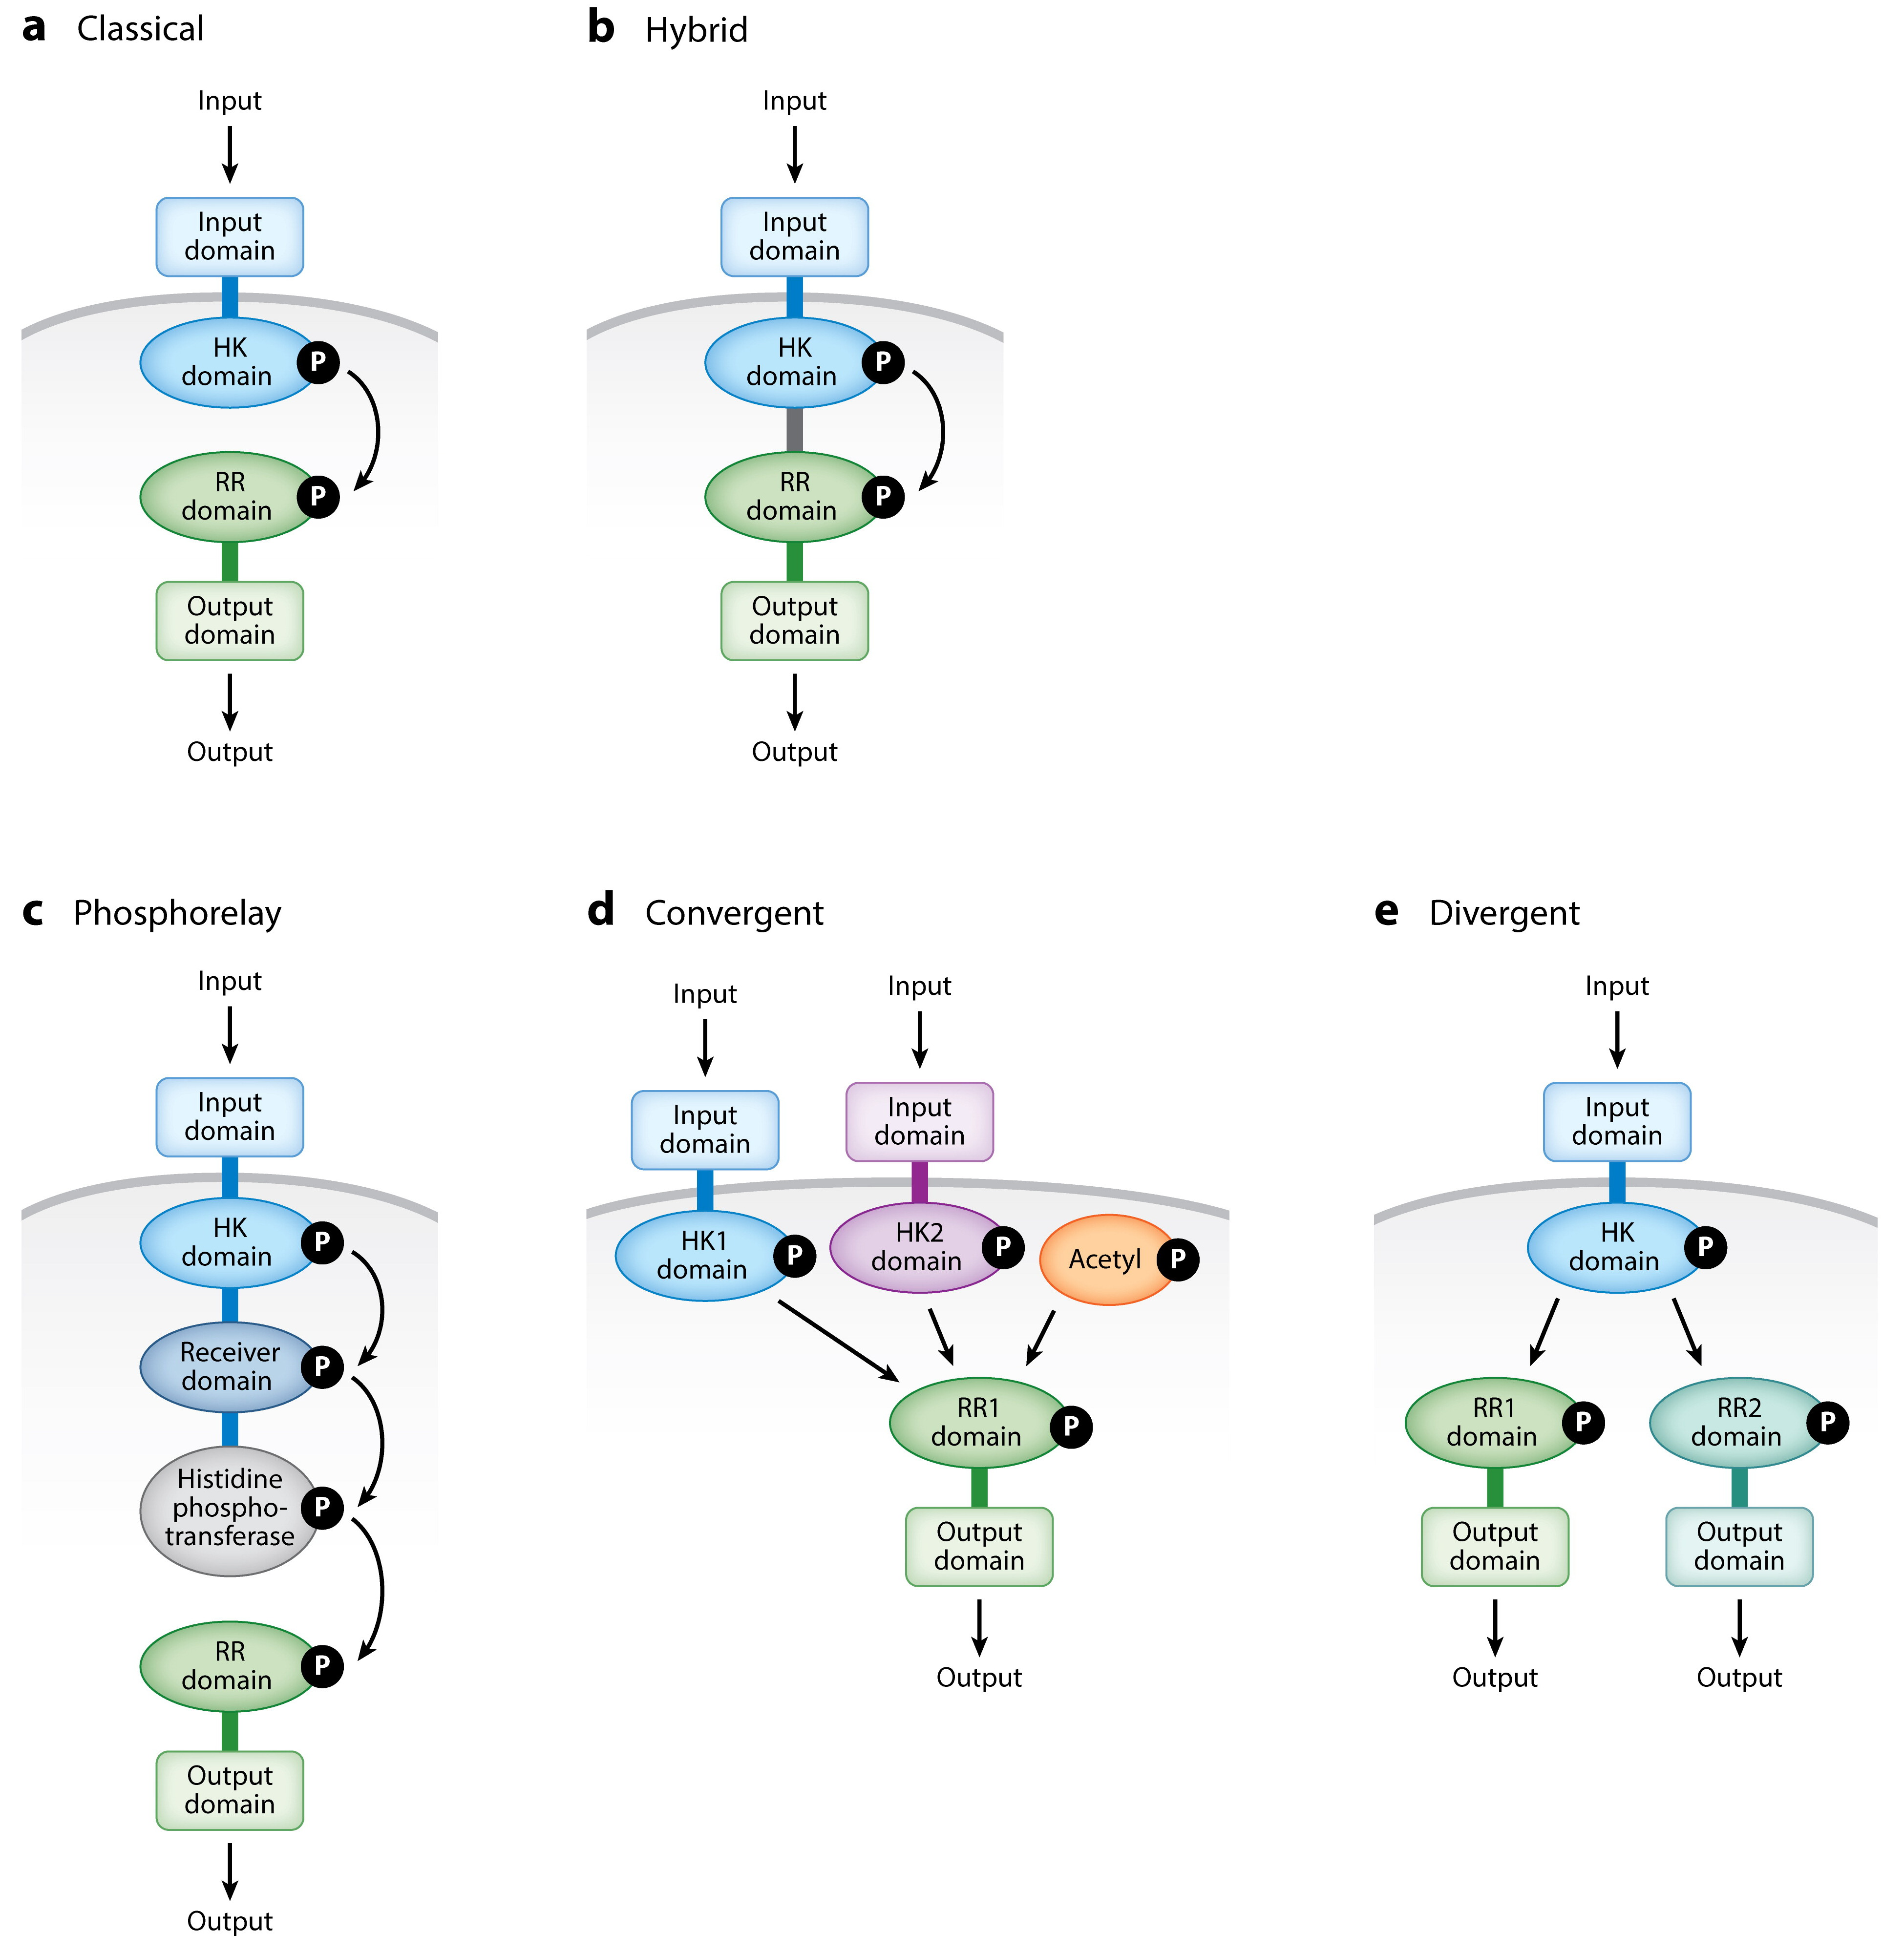
\includegraphics[scale=0.85]{text/Pictures/TwoComponent.jpeg}
	\caption{Two-component signaling pathways. \textbf{a} histidine kinase (HK) autophosphorylates in response to a signal and subsequently transfers the phosphate to a response regulator (RR) which generates output. \textbf{b} a hybrid system comprises both components (HK and RR) into a single protein. \textbf{c} in phosphorelay the phosphate is transferred multiple times before reaching its final RR. \textbf{d} some RR can be activated by several HK including metabolites such as acetyl phosphate. \textbf{e} one HK might phosphorylate multiple RR generating various outputs. (reproduced from \cite{groisman2016feedback})}
	\label{two}
\end{figure}

Another version of two-component system is phosphorelay (Fig. \ref{two}\textcolor{red}{c}).
In this case multiple steps of phosphate transfer occur before the final phosphorylation of target regulator.
Histidine domain of sensor protein serves here as a phosphate donor to an aspartate domain of the same or another protein.
From this domain the phosphate is further transferred to another histidine domain.
This can exist again within the same protein or as a separated one.
And finally, the aspartate domain of a DNA-binding regulator receives phosphate from the third domain in row.
These multiple steps allow easier regulation by other signals as the phosphorelay can be silenced at any of the intermediate steps during the transmission \cite{perego2001pentapeptide, groisman2016feedback}.

Systems where a regulatory protein can be phosphorylated by different sensory units also occur.
And even phosphorylated metabolites might act as signal donors (Fig. \ref{two}\textcolor{red}{d}).
This results in similar outputs in response to various signals \cite{kaczmarczyk2014complex, chambonnier2016hybrid}.

Contrary, some cases require various response to a single signal, when multiple genes are affected.
A divergent signal transmission mediates this (Fig. \ref{two}\textcolor{red}{e}) as one sensory kinase is able to phosphorylate aspartate domains of different acceptor proteins \cite{mika2005two, groisman2016feedback}.
Moreover, all these variations of two-component system mentioned above combine in cells producing a complex sensory-response network \cite{kaczmarczyk2014complex, chambonnier2016hybrid}.
%%% should i describe the responses more in detail?

\subsection{Bacterial gene regulation}
As mentioned above several ways of control of gene products take place in bacterial cells.
Regulation of translation in bacteria is a useful tool for controlling differential production of proteins coded within the same operon and thus transcribed on the same mRNA \cite{dar2018extensive}.
In the case of enzymes responding to quick changes it is useful to have those prepared in the cell even if not in use at the time.
% 2018.07.12 might be useful to give some indication of the time scale for thee pathways, eg transciption speed, mRNA half life, protein half life. e.g. if you want to react in seconds you can't depend on txn and tln, but if you need to react in minutes/hours it's fine.
When it comes to a sudden change in the environment the cell doesn't need to wait until the protein is transcribed and translated, but it only releases the activity of such protein.
Histidine kinases of two-component system mentioned above serve as a good example.
Transcriptional regulation on the other hand might be considered as the most economical as it inhibits the very synthesis of products which are not needed at the moment.
This saves resources and energy for synthesis of desired gene outputs.
The last mentioned type of regulation is delineated further in detail.
%%% Add more references?

\subsubsection{DNA accessibility}
Having coding sequence and promoter of certain gene physically accessible for specific transcription regulation is one of the prerequisites of its expression.
Nucleoid associated proteins (NAPs) and supercoiling are general mechanisms affecting this accessibility.
NAPs' role in several cell processes such as replication, horizontal gene transfer or transcription regulation was shown \cite{dixon1984protein, kayoko1992histone, aznar2013hha}.
Here I mention principally their global influence of gene expression and respective DNA accessibility to other DNA-binding transcriptional factors and RNA polymerase.
NAPs in general have dual effect on transcription i.e. can act as both enhancers or silencers of genes.

H-NS is one of the most abundant nucleoid-associated proteins of \textit{E. coli} chromosome which occur at all growth phases \cite{azam1999growth}.
Its expression is negatively autoregulated, but another NAP Fis acts as an activator of \tax{hns} gene \cite{ueguchi1993autoregulatory, falconi1996antagonistic}.
H-NS binds AT-rich DNA regions and forms polymers bridging distant DNA sequences  \cite{navarre2006selective, arold2010h}.
This leads to promoter silencing especially in cases when $\alpha$ subunit of RNA polymerase uses AT-rich sites to stabilize binding of the whole complex to the promoter \cite{singh2013h}.
However H-NS can compete with RNA polymerase and other transcriptional factors binding of AT-rich sites in general.
RNA polymerase might get even stuck in a DNA loop unable to elongate mRNA \cite{dame2002structural}.
Creation of such loops is the outcome of H-NS polymerization.
The silencing of affected promoters is not strict though as RNA polymerase sometimes bypasses this by association with an alternative $\sigma$ factors instead of conventional $\sigma^{70}$ \cite{grainger2008selective}.
Although H-NS is generally considered as global gene silencer an evidence of H-NS requirement for successful transcription initiation was published \cite{singh2013h}.

Fis protein similarly to H-NS prefers binding of AT-rich sites and is negatively autoregulated \cite{ball1992dramatic, stella2010shape}.
Fis's ability to affect gene expression in both positive and negative way is better known \cite{choi2005effects, karambelkar2012silencing}.
Moreover it antagonizes H-NS silencing of some promoters \cite{falconi2001involvement}.
Even though Fis shares its binding preferences for AT-rich DNA with H-NS, it doesn't polymerase but bends the DNA sequence at the binding site \cite{hubner1989bent}.
This bending is essential for e.g. transcription initiation of ribosomal gene \tax{rrnB} \cite{gosink1993dna}.

These two NAPs described here belong among the ones which are most understood these days and don't represent an exhaustive outline of all bacterial NAPs.
Review from 2010 lists 14 additional bacterial NAPs \cite{dillon2010bacterial}, but even their list is not complete \cite{aznar2013hha}.

At the end of this block I'd like to mention supercoiling which also affects the access to the genetic code \cite{brahms1985activation}.
Overwinding (positive supercoiling) and underwinding (negative supercoiling) is generated during transcription when transcription bubble forms \cite{wu1988transcription}.
This happens thanks to the helical structure of DNA.
Although some NAPs such as Fis and H-NS might affect the supercoiling levels \cite{ouafa2012nucleoid} topoisomerases take care of this process.
\tax{E. coli} possess two major topoisomerases - gyrase (topoisomerase II) and topoisomerase I.
The former releases positive the latter negative supercoiling \cite{wang1971interaction, gellert1976dna}.
If high levels of supercoiling are not released the access to the DNA reduces and even already initiated transcription is slowed down or terminated \cite{chong2014mechanism}.
%%% Add references!!!

\subsubsection{Transcription initiation}


\subsubsection{Elongation of mRNA}


\subsubsection{Transcription termination}


\subsection{Epigenetic mechanisms in bacteria}
Epigenetics is understood as a heritable change in gene expression without simultaneous changes in DNA primary sequence.
Various epigenetic mechanisms such as histone modifications, genomic imprinting or RNA associated silencing are well studied in eukaryotes \cite{durso2014mechanisms}.
In bacterial domain DNA methylation by methyltransferases is mostly mentioned, although positive and double negative feedback loops play their role as well especially in terms of population bistability \cite{casadesus2006epigenetic, casadesus2013programmed, adhikari2016dna}.

\subsubsection{DNA methylation by orphan methyltransferases}
Orphan methyltransferases (MTs) were initially studied within restriction-modification system as a bacterial defence against phages, although Dam's ability to alter some gene expression was already described in mid-80s \cite{sternberg1985evidence, bickle1993biology}.
As orphan MTs lack their cognate restriction endonucleases their role in bacterial cells is not as a primitive immune system, but among others can act as a transcription regulators.
I describe the epigenetic mechanisms of Dam in detail below as the MT whose relationship to cell memory is most understood.
Some authors consider the change in expression of certain genes in \tax{Caulobacter crescentus} which is associated with an orphan MT called CcrM to be epigenetic as well \cite{casadesus2006epigenetic, adhikari2016dna}.
However I do not include it here as these transcriptional changes are not heritable and occur only during a part of cell cycle.
Other \tax{E. coli} orhan MTs are mentioned briefly as well although none of them is known to play a role in epigenetics so far.

\textbf{Dam}, one of two first orphan MTs described in \tax{E. coli}, methylates adenine in 5'-GATC-3' sequences to N$^6$-methyladenine (6mA) \cite{marinus1973isolation}.
Its homologs were found in some bacteriophages as well as in other \tax{Gammaproteobacteria}, however many of bacterial DNA adenine methylases are associated with restriction endonucleases \cite{low2001roles, casadesus2006epigenetic, bochow2012bacteriophage}.
On the other hand strains having an orphan DNA adenine methylase can be characterized by presence of SeqA and MutH, overrepresentation of GATC sites in \tax{oriC}, genes close to it and in the \tax{dnaA} promoter \cite{sobetzko2016distamo}.
For most of the DNA both strands of chromosome are fully methylated throughout the cell cycle if Dam is present.
Of course, one of the exceptions is a short time hemimethylation of a leading strand and Okazaki fragments right after their synthesis during replication.
Both strands lack GATC methylation in \tax{dam} mutants, moreover higher mutation rate, uncoordinated replication initiation or loss of virulence were observed as well.
Interestingly for some species e.g. \tax{Vibrio cholerae} the presence of an orphan DNA adenine methylase is vital, whereas it is non-essential for other, such as \tax{E. coli} \cite{casadesus2006epigenetic, casadesus2013programmed, adhikari2016dna}.

As implied above several GATC sites escape Dam methylation.
This happens if another regulatory protein recognises a specific DNA biding site which overlaps GATC sequence and thus competes with Dam for it \cite{correnti2002dam}.
Such mechanism leading to epigenetic switch is well characterized in synthesis of \tax{pap} pili in uropathogenic \tax{E. coli} (UPEC) \cite{peterson2008competitive}.
The regulatory sequence of the \tax{pap} operon contains two sets of Lrp binding sites 1-3 and 4-6.
In both of them GATC sequence is present, GATC$^{prox}$ within site 2 and GATC$^{dist}$ within site 5 (Fig.~\ref{pap}) \cite{blyn1990regulation}.
%%% is this picture better? or is it too simple?
\begin{figure}[h!]
  \centering
  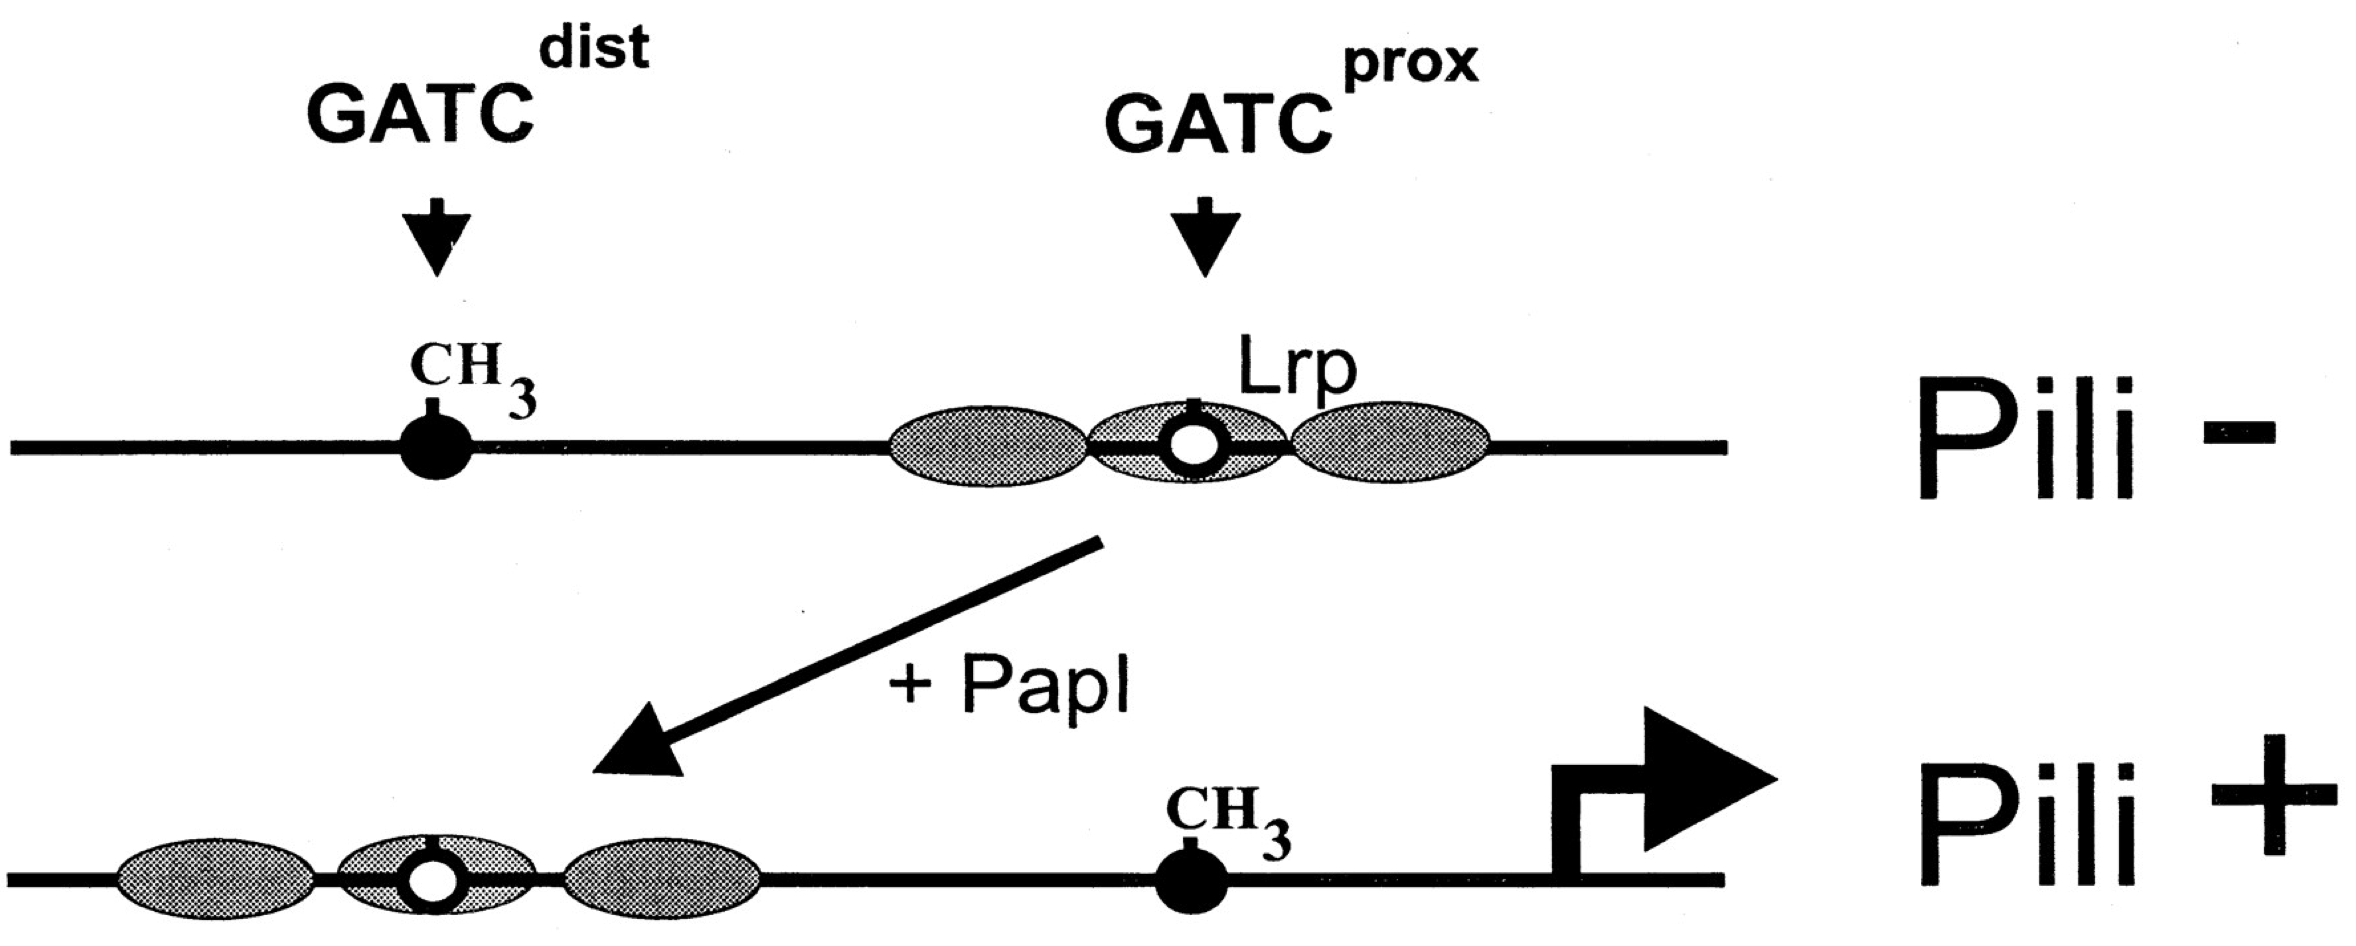
\includegraphics[scale=0.3]{text/Pictures/papPili.png}
	\caption{Scheme of the \tax{pap} phase OFF to ON switch. (reproduced from \cite{low2001roles})}
	\label{pap}
\end{figure}
During the OFF phase \tax{pap} pili are not produced because Lrp occupies GATC$^{prox}$ site which remains nonmethylated on both strands while GATC$^{dist}$ is fully methylated.
Lrp in this position prevents binding not only by Dam but by $\sigma^{70}$ RNA polymerase as well inhibiting expression of \tax{papBA} gene \cite{weyand2000regulation}.
For switch to ON phase an initial Lrp dissociation from sites 1-3 is necessary.
This likely happens during replication when an opportunity for Lrp to bind the hemimethylated GATC$^{dist}$ site instead of GATC$^{prox}$ raises.
The probability of this switch depends on the level of regulatory protein PapI in the cell as complex PapI/Lrp has lower affinity to site 2 but binds more likely to hemimethylated sites 4-6 than to fully methylated DNA \cite{hernday2003mechanism}.
Besides Lrp release from GATC$^{prox}$ site enables access of Dam to it so it can become methylated which further reduces Lrp affinity to 1-3 sites.
Even though RNA polymerase's access to \tax{papBA} promoter is not blocked any more the expression itself requires cAMP-CAP \cite{weyand2001essential}.
When PapB is beeing produced it acts as a \tax{papI} gene transcription activator leading to a feedback loop which stabilizes the cells in ON phase \cite{forsman1989autoregulation}.
However the described transition from OFF to ON phase occurs with 100-fold lower frequency than vice versa \cite{blyn1990regulation}.
The process of this opposite transition i.e. from ON to OFF phase involves transfer of Lrp from GATC$^{dist}$ to GATC$^{prox}$ during replication but the exact mechanism is not fully understood yet \cite{adhikari2016dna}.

Another well known orphan MT in \tax{E. coli} is \textbf{Dcm} which methylates second cytosine in 5'-CC(A/T)GG-3' motif to 5-methylcytosine (5mC) \cite{marinus1973isolation}.
Even though neither this one is necessary for \tax{E. coli} survival and some strains were found lacking \tax{dcm} gene, link between certain genes expression and presence of this MT was described.
Dcm seems to slow down expression of ribosomal genes \tax{rplC} and \tax{rpsJ} and inhibit transcription of \tax{sugE} gene connected with higher antimicrobial resistance \cite{militello2012conservation, militello2014cytosine}.
Both is happening predominantly during early stationary phase.
Next study shows increased expression of stress response sigma factor RpoS in \tax{dcm} mutant \cite{kahramanoglou2012genomics}.
Recently additional 63 genes were discovered to be affected if Dcm activity is inhibited \cite{militello20165}.
Most of these genes are up-regulater during early stationary phase if methylation by Dcm is silenced.

Lastly \textbf{YhdJ} is an orphan MT methylating 3' adenine of 5'-ATGCAT-3' sequence to 6mA when overexpressed.
Deleting \tax{yhdJ} gene produces neither loss of viability of \tax{E. coli} nor changes in its phenotype.
In addition, the expression of the gene is very low under usual laboratory conditions and nothing is known about transcription regulation of the gene \cite{broadbent2007yhdj}.

% 2018.06.28
% Eventually, go into way more detail here, as this will end up as a full section on lac. But if you are leaving this as a brief intro to positive, negative, double negative, that's fine. You might also start with sensing/reaction and then move to epigenetics. This is a reasonable ref I think *An introduction to systems biology: design principles of biological circuits*, although you always have to be a little careful with Uri Alon's take on things, sometimes it's a bit too facile.
\subsubsection{Feedback loops}
System where a product is able to affect positively or negatively its own production is called a feedback loop.
The influence of the output on itself might be direct or indirect if multiple effectors are involved.
Feedback loops are quite common in bacterial gene regulation and can lead to epigenetic switches \cite{smits2006phenotypic, veening2008bistability}.
Positive feedback loop and double negative feedback loop are known to play a role in memory of prokaryotes so far and are characterized in detail below.

\textbf{Positive feedback loop} is the first described example of bacterial epigenetics.
It was shown already in 1957 that \tax{E. coli} sub-population primed by high concentration of lactose analogue TMG is able to maintain \tax{lac} operon fully induced even in low non-inducible TMG concentrations \cite{novick1957enzyme}.
While if the same bacteria are exposed to the low non-inducible TMG concentration without priming the \tax{lac} operon remains repressed by LacI.
The mechanism behind this resides in different levels of $\beta$-galactoside permease (LacY) in TMG induced and naive cells.
Induced population has high level of the permease present in membrane as \tax{lacY} gene expression is activated by high TMG concentrations.
This state is preserved in a sub-population of induced cells after transfer into low TMG concentration as the abundant permease is able to maintain intracellular TMG level high enough to avoid LacI repression.
Thus the high level of permease leads to high intracellular TMG concentration which in turn acts as permease transcription activator.
On the other side naive cells have very small amounts of LacY if any thus they are not able to obtain TMG from the solution to activate \tax{lac} operon expression \cite{smits2006phenotypic, casadesus2013programmed}.

\begin{figure}[h!]
  \centering
  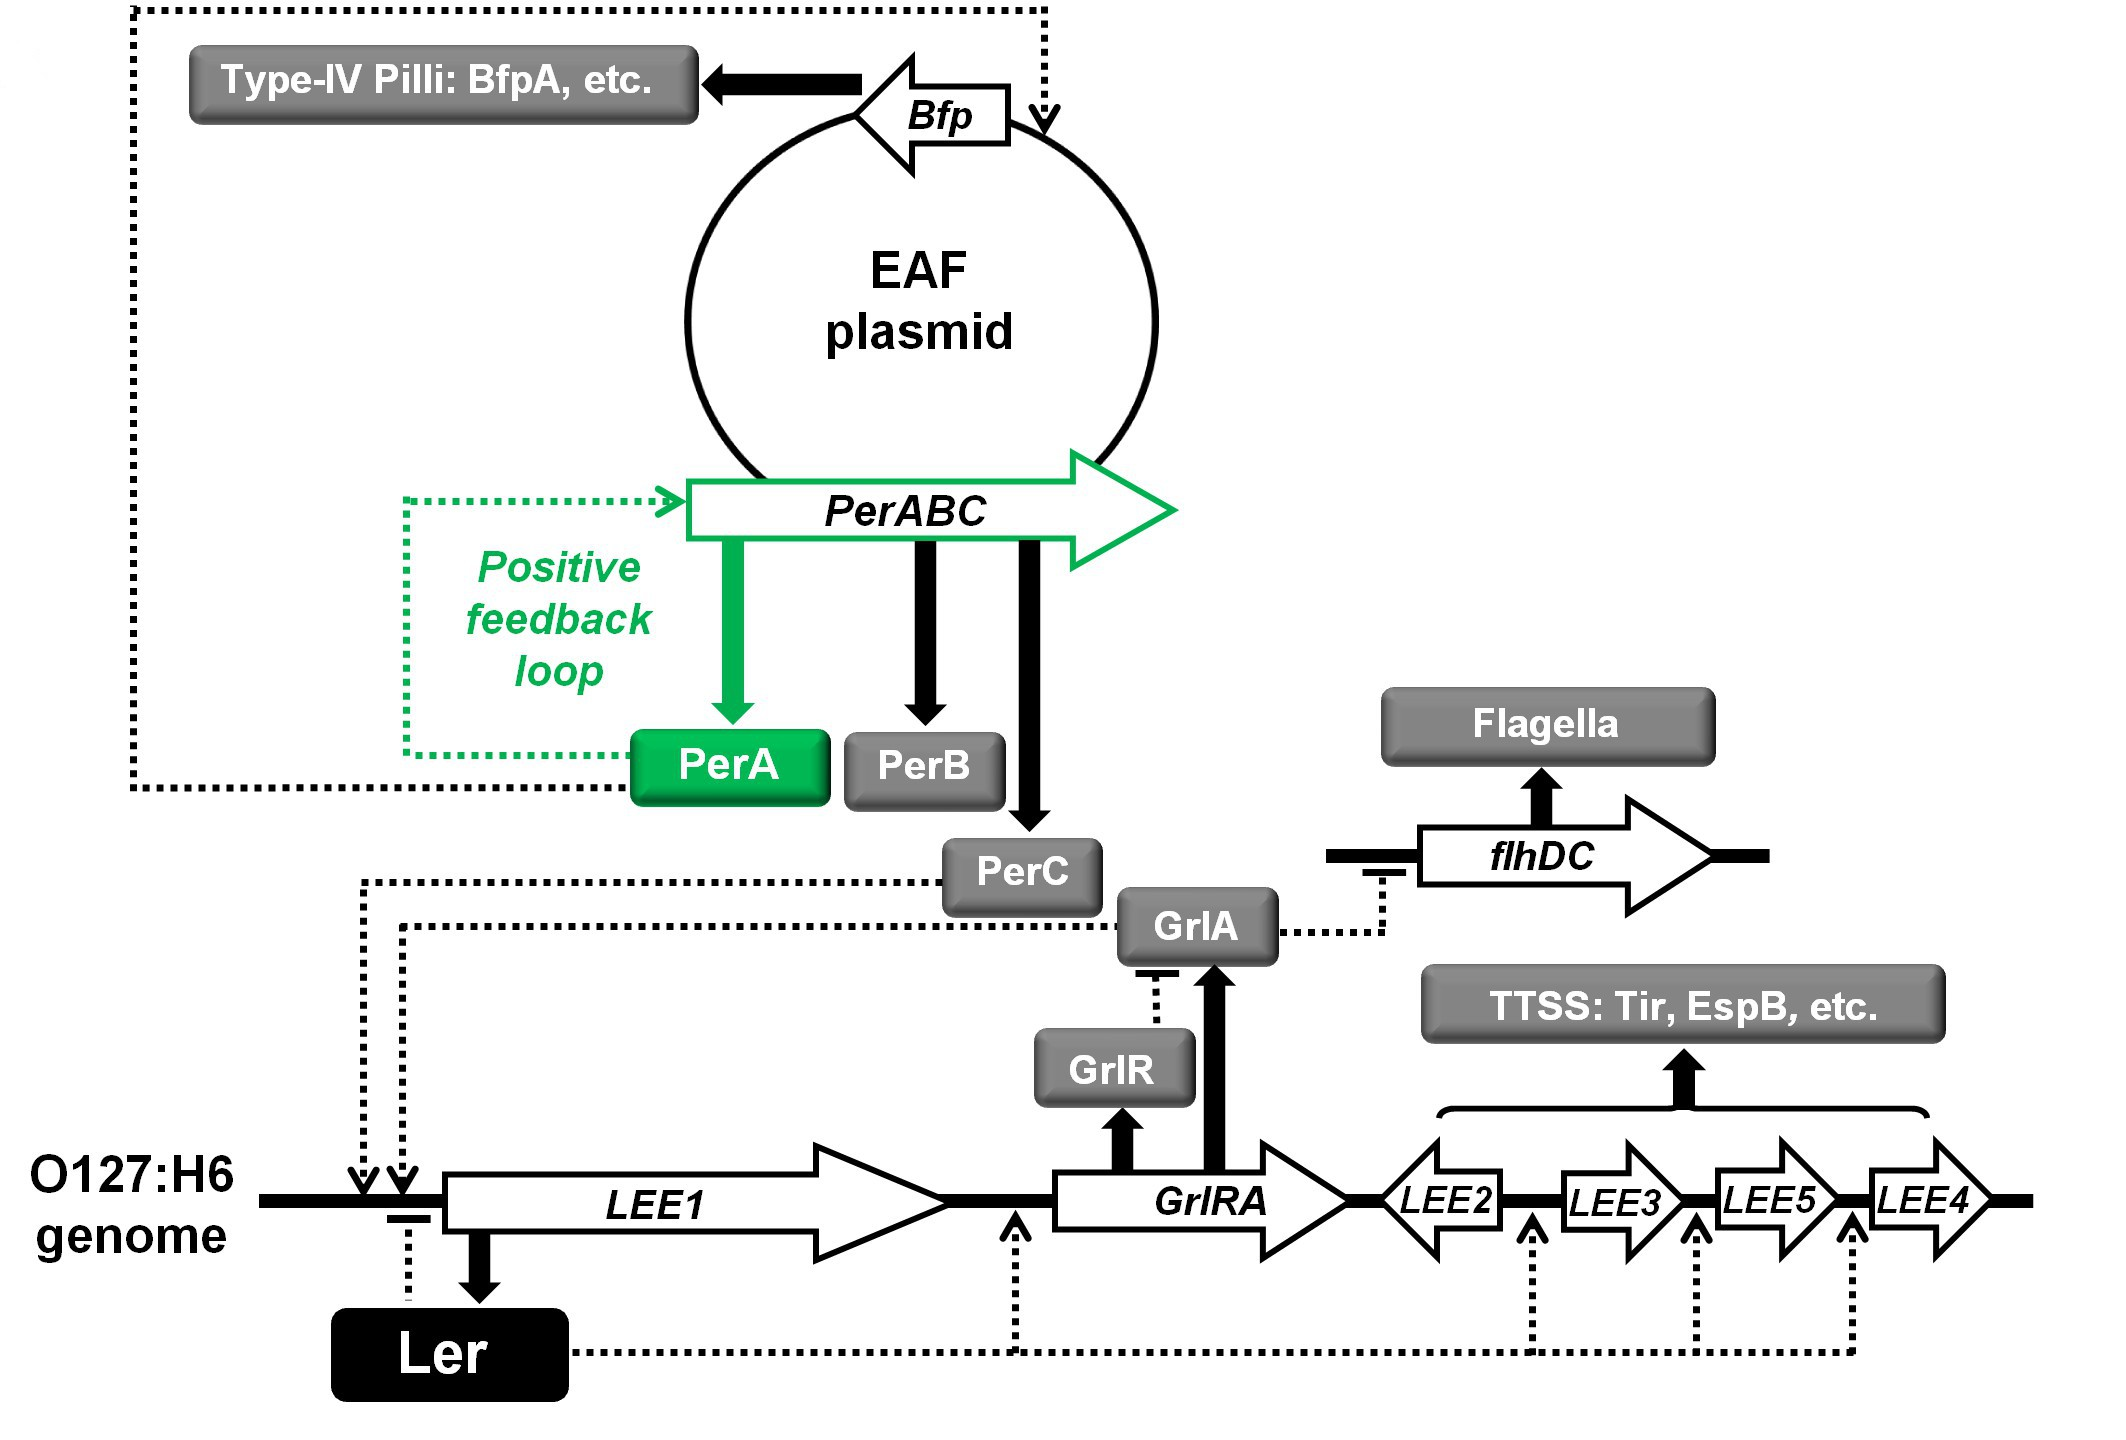
\includegraphics[scale=0.2]{text/Pictures/perOperonRegulation.jpg}
	\caption{Scheme of EPEC virulence regulation. PerA positivelly autoregulates \tax{perABC} operon and the triggers expression of type IV pili. PerC activates transcription of Ler which is the main regulator of T3SS secretion system machinery. (reproduced from \cite{ronin2017long})}
	\label{per}
\end{figure}

Another nice example of a long-term virulence epigenetic switch mediated by a positive feedback loop was published last year.
Enteropathogenic \tax{E. coli} (EPEC) coexists in two, non-virulent and hyper-virulent, sub-populations during growth \cite{ronin2017long}.
This bimodality was first observed  using ScanLag \cite{levin2014scanlag} as a difference in growth rates of the two groups resulting in BIG and SMALL colony morphotypes, for early and late appearing colonies, respectively.
In transcription level it is a change in \tax{per} operon expression (located on EAF plasmid) and \tax{per} regulated genes.
EPEC cultivation in virulence-activating conditions gives rise to \tax{per}-ON hyper-virulent aggregative sub-population (SMALL phenotype) reaching nearly 100\% \cite{ronin2017long}.
Interestingly this high ratio of \tax{per}-ON vs \tax{per}-OFF cells remains for many generations even after transferring the culture back into non-activating conditions, although naive EPEC culture contains only a minority of \tax{per}-ON cells.
Transition back from \tax{per}-ON to \tax{per}-OFF phase is achieved when cells are grown up to stationary phase.
The long-term stability of \tax{per}-ON state relies on a positive feedback of PerA which acts as an activator of its own gene beside \tax{perB} and \tax{perC} in the \tax{per} operon (Fig.~\ref{per}) \cite{ibarra2003identification, ronin2017long}.
%%% More examples of positive feedback to add???

As an illustration of \textbf{double negative feedback loop} in epigenetic regulation a switch between lytic and lysogenic cycle of \tax{E. coli} phage $\lambda$ is often described \cite{smits2006phenotypic, casadesus2013programmed}.
After inserting its DNA the virus cycle might undergo two different ways - i.e. either replicate producing a lot of new phages and heading for bacterial lysis or integrate its own DNA into the bacterial chromosome and persist there within a lysogeny.
The fate of the phage lies in two repressors, CI and Cro, each repressing transcription of the other \cite{eisen1970regulation, neubauer1970immunity}.
Besides CI inhibits phage propagation genes and activates its own transcription.
However, both CI and Cro are produced since the beginning of the infection.
If the level of CI reaches a certain threshold and outcompetes Cro, whose activity is suppressed, the phage enters a lysogenic cycle staying dormant in the cell thanks to CI-\tax{cI} positive feedback loop.
Otherwise Cro levels rise further inhibiting CI production and establishing phage proliferation with subsequent cell lysis \cite{svenningsen2005role}.
It should be noted that although it is not predictable whether the phage enters lytic or lysogenic cycle, the ratio of lysed/lysogenized cells depends on bacterial physiologic situation and other environmental factors as well.
Interestingly, Toman et al. used the CI-Cro system for epigenetic reuglation of \tax{gal} operon in \tax{E. coli} \cite{toman1985system}.
%%% it's not epigenetics in E. coli, but in the phage lambda! (except for the engineered system by Toman et al.)

%%%As the CI-Cro regulation is a phage system, the first evidence of bacterial epigenetics driven by a double negative feedback loop was published just 3 years ago.

%%% detection of double negative feedback loop originating in bacteria?
%%% double negative feedback detected in "A Novel Feedback Loop That Controls Bimodal Expression of Genetic Competence" which talks about cell competence
%%% there is no direct evidence for epigenetics playing role in it, however paper "Agent-based modeling of competence phenotype switching in Bacillus subtilis" suggests it might be so according to their model
%%% especially when in similar case - bacillus sporulation is it proven in: "Bet-hedging and epigenetic inheritance in bacterial cell development"


%%% swapped paragraph from 0.1 Taxonomy and characteristic of E. coli
Although the presence of \tax{E. coli} in water is still widely used as an indicator of fecal contamination recent studies show that some \tax{E. coli} isolates are able to  reproduce in soil \cite{byappanahalli2004indigenous, somorin2016general}.
Moreover strains inhabiting soil for a long time were found to be distinctive \cite{walk2009cryptic, walk2015cryptic}.
This raises the questions how these bacteria survive outside their hosts and how do they evolve under such conditions.




\cleardoublepage

